\section{Tracing and Monitoring of Control-Flow}

The tracing and monitoring of control-flow is perhaps the most important element of any CFI solution, as all control-flow change events need to be captured in order to ensure CFI. One method of capturing control-flow is through software, where functions are written and APIs provided which intercept control-flow events. Another method is to add dedicated hardware into the processor pipeline, where it intercepts each instruction (when the instruction is retrieved from memory prior to execution).

\subsection{Granularity of Monitoring}\label{implementationGranularity}

If a software-only method were to be used, recording of every executed instruction is infeasible as the overhead added would be too large (if no additional hardware is included), as each instruction processed would require a corresponding context switch and further processing. If each instruction is hashed in real time the computational overhead would increase or, if each instruction is recorded in storage prior to processing the memory\slash storage\slash IO, capacity would see a significant overhead increase. The use of basic blocks allows us to deal with multiple instructions at a time, and therefore reduce the potential overheads dramatically.

CFG granularity can be broken down into three levels \cite{Abera2016}:
\begin{enumerate}
	\item{Entire functions}
	\item{Basic Blocks ending in a direct branch (this would cover most ROP attacks)}
	\item{Basic Blocks ending in any branch instruction (providing the highest level of detail)}
\end{enumerate}

To achieve the best coverage for the proposed solution, level 3 (basic Blocks ending in any branch instruction) would be the optimum granularity to aim for. We have taken inspiration from C-FLAT\cite{Abera2016} when considering the design for the proposed solution, as it most closely aligns with the objectives of this project.

\subsection{Representing the Execution Path}

We can build up a hash of the flow by taking the ID (or memory address) of the source node and hashing that with the previous hash. At the start ($ID_1$) the previous hash would be replaced with zero, a nonce or a hash created as part of the static attestation process. The resulting chain would appear as: 
$H_1 = H(ID_1,0)$ (or $H_1 = H(ID_1,nonce)$), $H_2 = H(ID_2,H_1)$ \ldots $H_n = H(ID_n,H_{n-1})$.

\begin{figure}
  \centering
  \vspace*{0.5in}
  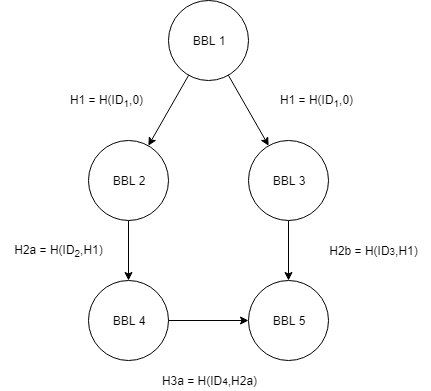
\includegraphics[scale=0.5]{CFGhash.png}
  \caption{Construction of a control-flow hash}
  \label{fig:controlFlowHash}
\end{figure}

Figure~\ref{fig:controlFlowHash} demonstrates how a hash would be constructed along two different control-flow paths. Even though execution flows through BBL5 in both paths, the hashes would be different as they have been constructed from different sets of hashes.

The hash function implemented would be BLAKE2 \cite{Aumasson2013}, as it is a lightweight and a widely used hash function with many supported implementations in different programming languages (meaning the embedded code could use its C implementation while the CFG building application could use its Python implementation).

To trigger the saving of the execution path hash, the proposed solution would implement a dedicated method in the secure world where a save is triggered, this will be exposed to software developers through the proposed solution's API. This functionality will enable software authors an opportunity to save at key points - for example after a key decision is made. The hash itself will be constructed by a measurement engine in the ``secure world''.

\subsubsection*{Challenges of CFG tracking}

Loops are a considerable issue with regard to tracking control flow, as the number of possible paths could be overwhelming, especially if the loops contain branch instructions or function calls.

To overcome the problems presented by loops, C-FLAT \cite{Abera2016} begins with treating loops as sub-programs. Where each run of a loop has a hash derived from it, and the total number of each time that hash was calculated is stored (therefore storing the number of times that exact sequence occurs). This has the potential to prove problematic, as a variety of paths through a loop could lead to a large number of combinations being stored. 

When this method was tested by C-FLAT \cite{Abera2016}, it was found that the resulting report was 1527 bytes for a path containing 16 loop invocations and 18 unique loop paths. Another path containing 12 loop invocations and 14 unique paths resulted in a 1179 byte result. A second study (which is not as well documented by the paper) produced a maximum result of 490 bytes. If an application were to present the opportunity for such a large number of loop variabilities, a warning could be presented at compile time.

Break statements need to be dealt with in a special manner as they are an additional place where a loop can exit. Section 4.2 of C-FLAT \cite{Abera2016} describes this in detail.

\subsubsection*{Instrumentation}

The instrumentation process allows us to modify the object code of the existing application in a manner which enables the monitoring of control-flow. In the case of the proposed solution, branches are identified and the destination address of the direct jumps are then added to the branch table. The destination addresses are then replaced with the address of the trampoline assembly code. 

The addition of trampoline assembly code enables redirecting execution to a single piece of simple and secure code without needing to add too many instructions during instrumentation. A trampoline may carry out a number of functions. For example, in C-FLAT \cite{Abera2016} it manages the return address register as well as the register holding the destination address for indirect branches. When executed, the trampoline will trigger the measurement engine, add the source and destination address to the hash chain, redirect the program counter to the corresponding destination entry on the branch table therefore finally continuing with the normal execution of the application.

\begin{figure}
  \centering
  \vspace*{0.5in}
  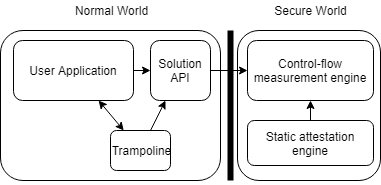
\includegraphics[scale=0.5]{GraphicalRepresentation.png}
  \caption{The systematic design of control-flow measurement in ARM TrustZone}
  \label{fig:graphicalRepresentation}
\end{figure}

Figure~\ref{fig:graphicalRepresentation} shows how trampolines are used to interface user applications with control-flow audit functionality. The figure also demonstrates how the API will expose the functionality of the measurement engine, and how the measurement engine takes input from the static attestation engine.